\documentstyle[11pt,epsfig,fancybox,semcolor,semlayer,doublespace,portrait]
{seminar}
\input clp_utils

\def\ys{$\Upsilon(1S)$}
\def\yss{$\Upsilon(2S)$}
\def\ysss{$\Upsilon(3S)$}
\def\gamee{$\Gamma_{e^+e^-}$}

% The following strings are needed by the title page and 
% page style definitions in map_utils.tex
\newcommand{\talktitle}[0]{\gamee for \ys, \yss\  and \ysss}
\newcommand{\fmttitle}[0]{}
\newcommand{\conftitle}[0]{May 2002 CLEO Meeting}
\newcommand{\myname}[0]{Jim Pivarski}
\newcommand{\affila}[0]{Cornell University}
\newcommand{\talkdate}[0]{May 11, 2002}

\pagestyle{conference}   % From clp_utils.tex

% slide magnification
\slidesmag 1

%%%%%%%%%%%%%%%%%%%%%%%%%%%%%%%%%%%%%%%%%%%%%%%%%%%%%%%%%%%%%%%%%%%%%%%%%%%
% Start document
\begin{document}

% Set page size
\slideheight 7.0in
\slidewidth 8.8in 

% Set array stretch
\renewcommand{\arraystretch}{0.3}
\renewcommand{\slidetopmargin}{0.4in}
\renewcommand{\slidebottommargin}{0.9in}


%%%%%%%%%%%%%%%%%%%%%%%%%%%%%%%%%%%%%%%%%%%%%%%%%%%%%%%%%%%%%%%%%%%%%%%%%%%

\begin{slide*}

\slideframe{}
\slideframe*[\dkblue]{Oval}

\begin{center}
\vspace{4 cm}
{\Huge \black \gamee\ for \ys, \yss\ and \ysss } \\
\epsfig{file=word_update.eps,width=\linewidth} \\
\vspace{1 cm}
{\LARGE \black	Jim Pivarski } \\
% \vspace{0.25 cm}
% {\LARGE	Ritchie Patterson } \\
% \vspace{0.25 cm}
% {\LARGE	Karl Berkelman } \\
\vspace{2 cm}
\conftitle \\
{\large \black \talkdate}

\end{center}

\end{slide*}

% %%%%%%%%%%%%%%%%%%%%%%%%%%%%%%%%%%%%%%%%%%%%%%%%%%%%%%%%%%%%%%%%%%%%%%%%%%%

% \begin{slide*}

% \slideframe{}
% \slideframe*[\dkblue]{Oval}
% \huge
% \heading{Outline}
% \vspace{1 cm}

% \begin{center}
% \begin{minipage}[t]{12 cm}
% \begin{itemize}
% \LARGE \item {\huge Motivation: verify lattice QCD!}
% \LARGE \item {\huge 2 out of 3 Resonances Scanned}
% \LARGE \item {\huge Energy Calibration Systematics}
% \LARGE \item {\huge Other Systematics / Work to be Done}
% \end{itemize}
% \end{minipage}
% \end{center}

% \end{slide*}
 
%%%%%%%%%%%%%%%%%%%%%%%%%%%%%%%%%%%%%%%%%%%%%%%%%%%%%%%%%%%%%%%%%%%%%%%%%%%

\begin{slide*}

\slideframe{}
\slideframe*[\dkblue]{Oval}
\huge
\heading{Outline}

\begin{minipage}[t]{\linewidth}
\LARGE

\begin{itemize}

  \item \yss\ data-taking has started.

  \item Energy calibration fluctuations $\le$ 0.2 MeV.

  \item I'm investigating cuts for hadron selection\ldots

  \item Efficiency can be measured from data:
        \begin{center} \ysss\ $\rightarrow$ \ys\ $\pi^+$ $\pi^-$. \end{center}

\end{itemize}

\end{minipage}

\end{slide*}

%%%%%%%%%%%%%%%%%%%%%%%%%%%%%%%%%%%%%%%%%%%%%%%%%%%%%%%%%%%%%%%%%%%%%%%%%%%

\begin{slide*}

\slideframe{}
\slideframe*[\dkblue]{Oval}
\huge
\heading{First \yss Scan}

\begin{minipage}[t]{\linewidth}
\LARGE

\vspace{1 cm}

\yss\ data-taking has begun!

\vspace{2 cm}

\begin{center}
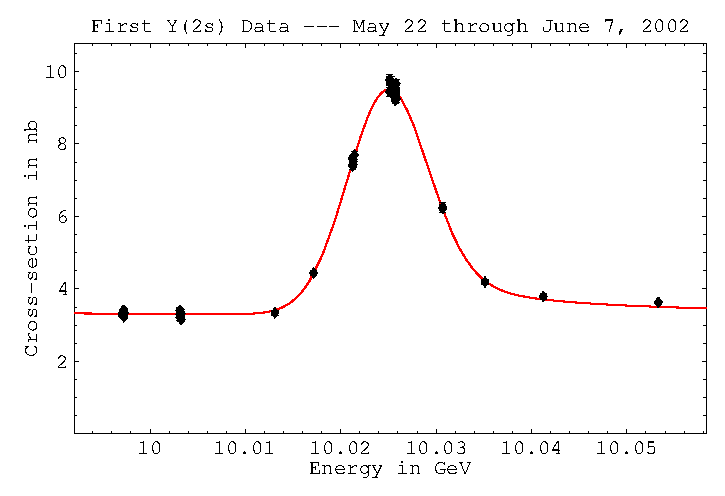
\epsfig{file=first_y2s.eps, width=\linewidth}
\end{center}

\end{minipage}

\end{slide*}

%%%%%%%%%%%%%%%%%%%%%%%%%%%%%%%%%%%%%%%%%%%%%%%%%%%%%%%%%%%%%%%%%%%%%%%%%%%

\begin{slide*}

\slideframe{}
\slideframe*[\dkblue]{Oval}
\huge
\heading{Energy Calibration Fluctuations}

\begin{minipage}[t]{\linewidth}
\Large

\begin{tabular}{p{0.4\linewidth} p{0.5\linewidth}}

\vspace{0.5 cm}

\begin{center}
  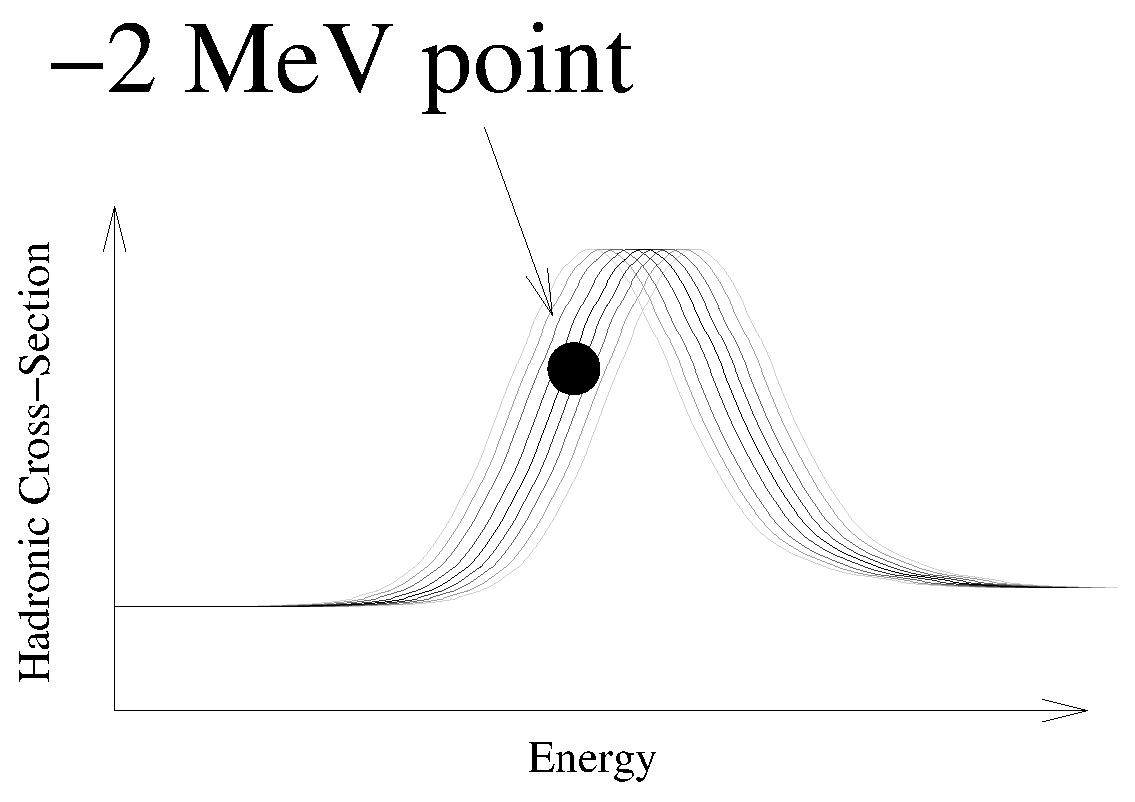
\epsfig{file=energy_wiggle.eps, width=0.85\linewidth}
\end{center}

\vspace{0.5 cm}

Repeatability of the \mbox{-2 MeV} energy point shows that the beam
energy program tracks energy changes in CESR to at least \mbox{$\pm$
0.2 MeV}.

\vspace{1 cm}

In \yss\ running, a larger data sample is being dedicated to the
\mbox{-2 MeV} point to try to constrain the fluctuations to
\mbox{$\pm$ 0.15 MeV} or lower.

  &
    \begin{center}
      \vfill
      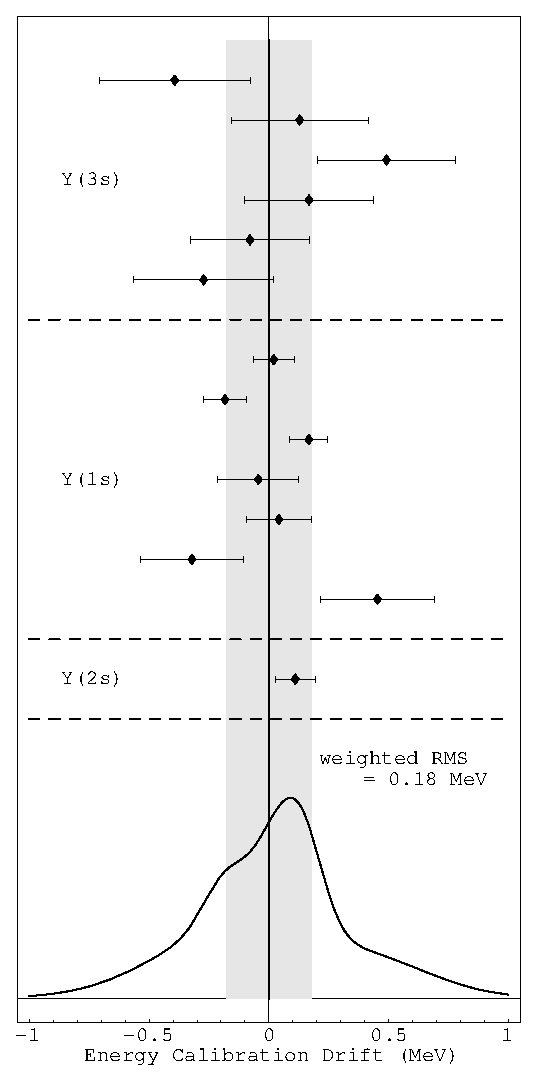
\epsfig{file=all_consistency.eps, width=\linewidth}
    \end{center} \\
\end{tabular}

\end{minipage}

\end{slide*}

%%%%%%%%%%%%%%%%%%%%%%%%%%%%%%%%%%%%%%%%%%%%%%%%%%%%%%%%%%%%%%%%%%%%%%%%%%%

\begin{slide*}

\slideframe{}
\slideframe*[\dkblue]{Oval}
\huge
\heading{Event Selection Cuts and Efficiency}

\begin{minipage}[t]{\linewidth}
\LARGE

We need a {\it very loose} set of cuts for an absolute measurement of
hadronic cross-section.

\vspace{0.5 cm}

They must cut out single-beam events and cosmics losing as few
beam-beam interactions as possible.

\vspace{0.5 cm}

Three promising variables:
\begin{itemize}

  \item {\bf event z0} = weighted average z0 position of all tracks in
  an event

  \item {\bf event d0} = weighted average $\big|$d0$\big|$ (radial)
  position of all tracks in an event

  \item {\bf bunchweight margin} =

\[ \frac{\mbox{best bunchweight score} - \mbox{second best}}{\mbox{best bunchweight score}} \]

  \begin{flushright} from TrackletBunchFinder. \end{flushright}

\end{itemize}

\end{minipage}

\end{slide*}

%%%%%%%%%%%%%%%%%%%%%%%%%%%%%%%%%%%%%%%%%%%%%%%%%%%%%%%%%%%%%%%%%%%%%%%%%%%

\begin{slide*}

\slideframe{}
\slideframe*[\dkblue]{Oval}
\huge
\heading{Event Selection Cuts and Efficiency}

\begin{minipage}[t]{\linewidth}
\LARGE

\begin{center}
  \vspace{-1 cm}
  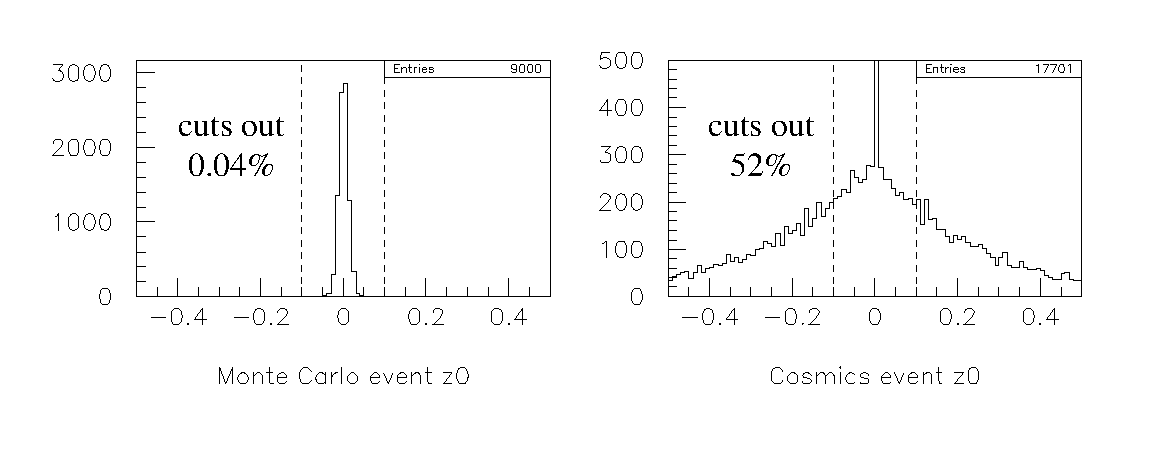
\epsfig{file=talk_wz0_2.eps,width=\linewidth} \\
  \vspace{-1 cm}
  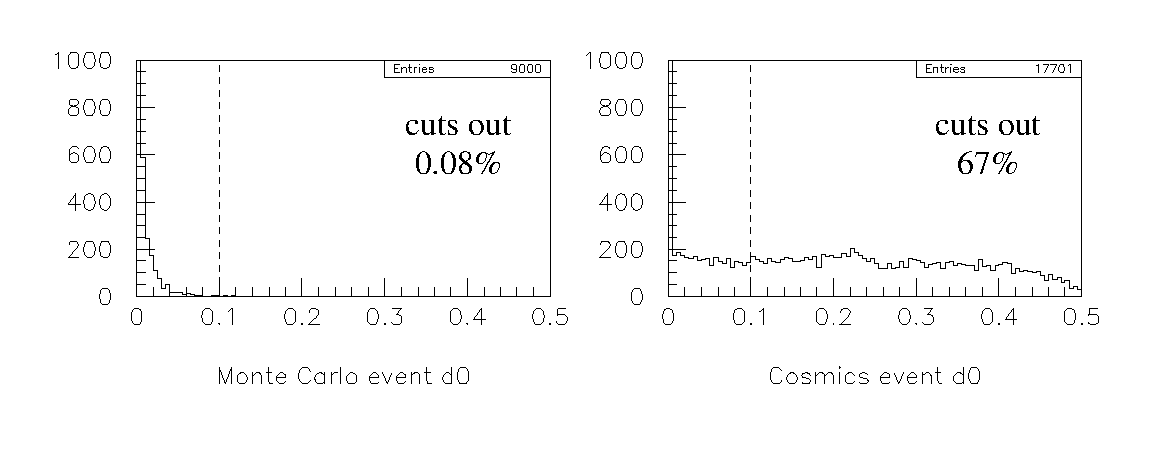
\epsfig{file=talk_wd0_2.eps,width=\linewidth} \\
  \vspace{-1 cm}
  \epsfig{file=talk_bunchweight_2.eps,width=\linewidth} \\

  The three cuts together remove $\sim$0.17\% of signal hadrons and
  73\% of cosmic ray background.

\end{center}

\end{minipage}

\end{slide*}

%%%%%%%%%%%%%%%%%%%%%%%%%%%%%%%%%%%%%%%%%%%%%%%%%%%%%%%%%%%%%%%%%%%%%%%%%%%

\begin{slide*}

\slideframe{}
\slideframe*[\dkblue]{Oval}
\huge
\heading{Event Selection Cuts and Efficiency}

\begin{minipage}[t]{\linewidth}
\LARGE

\vspace{0.5 cm}

Cut selection is a work in progress\ldots

\vspace{1 cm}

In order to study single-beam events (beam gas, beam wall, muon halo),
we will need a run taken with only one beam in the machine. Such a run
is scheduled to take place in the next few weeks.

\noindent\begin{tabular}{p{0.55\linewidth} p{0.025\linewidth} p{0.35\linewidth} p{0.025\linewidth}}

\vspace{1 cm}

\noindent ``Event d0'' can be replaced with a much tighter cut in X--Y. I will
start by trying the average of all helix crossings in 2--D.

& &
  \begin{center}
    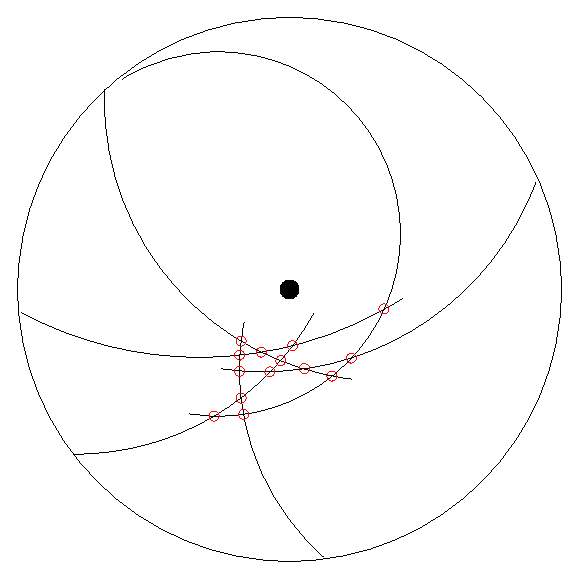
\epsfig{file=crossings_2d.eps,width=\linewidth}
  \end{center} \\
\end{tabular}

Something will have to be done with the no-track case.

\end{minipage}

\end{slide*}

%%%%%%%%%%%%%%%%%%%%%%%%%%%%%%%%%%%%%%%%%%%%%%%%%%%%%%%%%%%%%%%%%%%%%%%%%%%

\begin{slide*}

\slideframe{}
\slideframe*[\dkblue]{Oval}
\huge
\heading{Event Selection Cuts and Efficiency}

\begin{minipage}[t]{\linewidth}
\LARGE

\ys\ efficiency can be measured using data!

\begin{center}
  \epsfig{file=dipion_2.eps,width=\linewidth}
\end{center}

% \begin{tabular}{c c l}
%   $N_p$ &=& \ysss\ $\rightarrow$ \ys $\pi^+$ $\pi^-$ in ``peak''           \\
%   $N_{sb}$ &=& \ysss\ $\rightarrow$ \ys $\pi^+$ $\pi^-$ in ``side-band''   \\
%   $u_p$ &=& Events in $N_p$ sample which {\it fail} cuts                   \\
%   $u_{sb}$ &=& Events in $N_{sb}$ sample which {\it fail} cuts             \\
% \end{tabular}

% \[ \mbox{Efficiency} = 1 - \frac{u_p - u_{sb}}{N_p - N_{sb}} \]

% \[ \sigma_{\mbox{Efficiency}} = \sqrt{ \frac{u_p + u_{sb}}{(N_p - N_{sb})^2} +
%    \frac{(N_p + N_{sb})(u_p - u_{sb})^2}{(N_p - N_{sb})^4} } \]

Efficiency can be calculated as
\[ \epsilon = 1 - \frac{\mbox{events that fail cut: }
(\mbox{in peak} - \mbox{in side-band})}{\mbox{events: }
(\mbox{in peak} - \mbox{in side-band})} \mbox{.} \]

For 95\%--efficient cuts, statistical uncertainty is 0.5\%.

For 99\%--efficient cuts, statistical uncertainty is 0.2\%.

\end{minipage}

\end{slide*}

%%%%%%%%%%%%%%%%%%%%%%%%%%%%%%%%%%%%%%%%%%%%%%%%%%%%%%%%%%%%%%%%%%%%%%%%%%%

\begin{slide*}

\slideframe{}
\slideframe*[\dkblue]{Oval}
\huge
\heading{Conclusions}

\begin{minipage}[t]{\linewidth}
\LARGE

\begin{itemize}
  \item Data-taking is on schedule and the data looks good.
  \item Energy calibration is stable, so we're trying to tighten the bound.
  \item Tracking space and time cuts are good, but I'll need something more\ldots
  \item Our efficiency measurement can be Monte Carlo--independent.
\end{itemize}

\end{minipage}

\end{slide*}

%%%%%%%%%%%%%%%%%%%%%%%%%%%%%%%%%%%%%%%%%%%%%%%%%%%%%%%%%%%%%%%%%%%%%%%%%%%

\end{document}
